%%%%%%%%%%%%%%%%%%%%%%%%%%%%%%%%%%%%%%%%%%%%%%%%%%%%%%%%%%%%%%%%%%%%%%%%%%
\section{Hieroglyphen}
\index{Hieroglyphen}
%%%%%%%%%%%%%%%%%%%%%%%%%%%%%%%%%%%%%%%%%%%%%%%%%%%%%%%%%%%%%%%%%%%%%%%%%%
%

Der Standard f�r das Schreiben von Texten in \textit{toki pona} ist das lateinische Alphabet. 
Es wurden aber auch Schriftsysteme entwickelt, die auf Hieroglyphen basieren. 
Je nach System stellen die Symbole Buchstaben, Silben oder W�rter dar. 
Ein System, das f�r jedes Wort ein Symbol verwendet, ist \textit{sitelen pona} \cite{www:tokipona.org:02}.
Eine sehr sch�ne Hieroglyphenschrift hat Jonathan Gabel entwickelt. 
\textit{sitelen sitelen} \cite{www:jonathangabel.com:01} erinnert an Maya-Hieroglyphen.

Leider stellen die meisten dieser Systeme keine Satzzeichen und Sonderzeichen dar. 
Ein System, das auch Symbole f�r Satzzeichen hat ist \textit{sitelen pona pi jan Makuwe} \cite{www:janMakuwe:01}.
Diese Hieroglyphenschrift stellt Silben dar. 
Vokale werden als diakritische Zeichen auf die Konsonanten geschrieben, denen sie folgen.
Um ein 'n' am Ende einer Silbe zu schreiben, verwende einen Kreis in der Mitte des Symbols. 
Wenn die Silbe keinen Anfangskonsonanten hat, verwende einen Kreis mit einem senkrechten Strich.

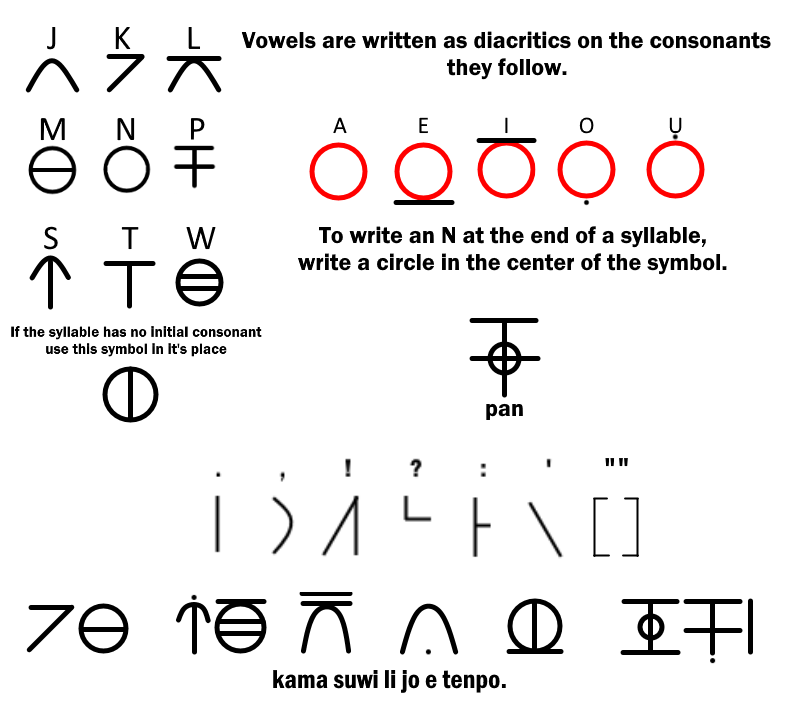
\includegraphics[scale=0.5]{sitelen_pona_pi_jan_Makuwe.png}

% 
%%%%%%%%%%%%%%%%%%%%%%%%%%%%%%%%%%%%%%%%%%%%%%%%%%%%%%%%%%%%%%%%%%%%%%%%%%
% eof
